Este capítulo dedica-se a explanar como a aplicação proposta para a intervenção ao problema, anteriormente descrito, executa suas ações e interações com outras aplicações. Para isso, é mostrado os fluxos e atividades de suas ações em figuras e descrito detalhadamente o que pode ser extraído das imagens.

\section{Diagrama de Atividade}

\begin{figure}[!htb]
        \caption{\label{diagrama1}Diagrama de Atividade}
        \begin{center}
                \includegraphics[width=\textwidth]{imagens/diagact.eps}
        \end{center}
        \legend{Fonte: Autor}
\end{figure}


\begin{figure}[!htb]
        \caption{\label{diagrama1}Fluxo de funcionamento da aplicação}
        \begin{center}
                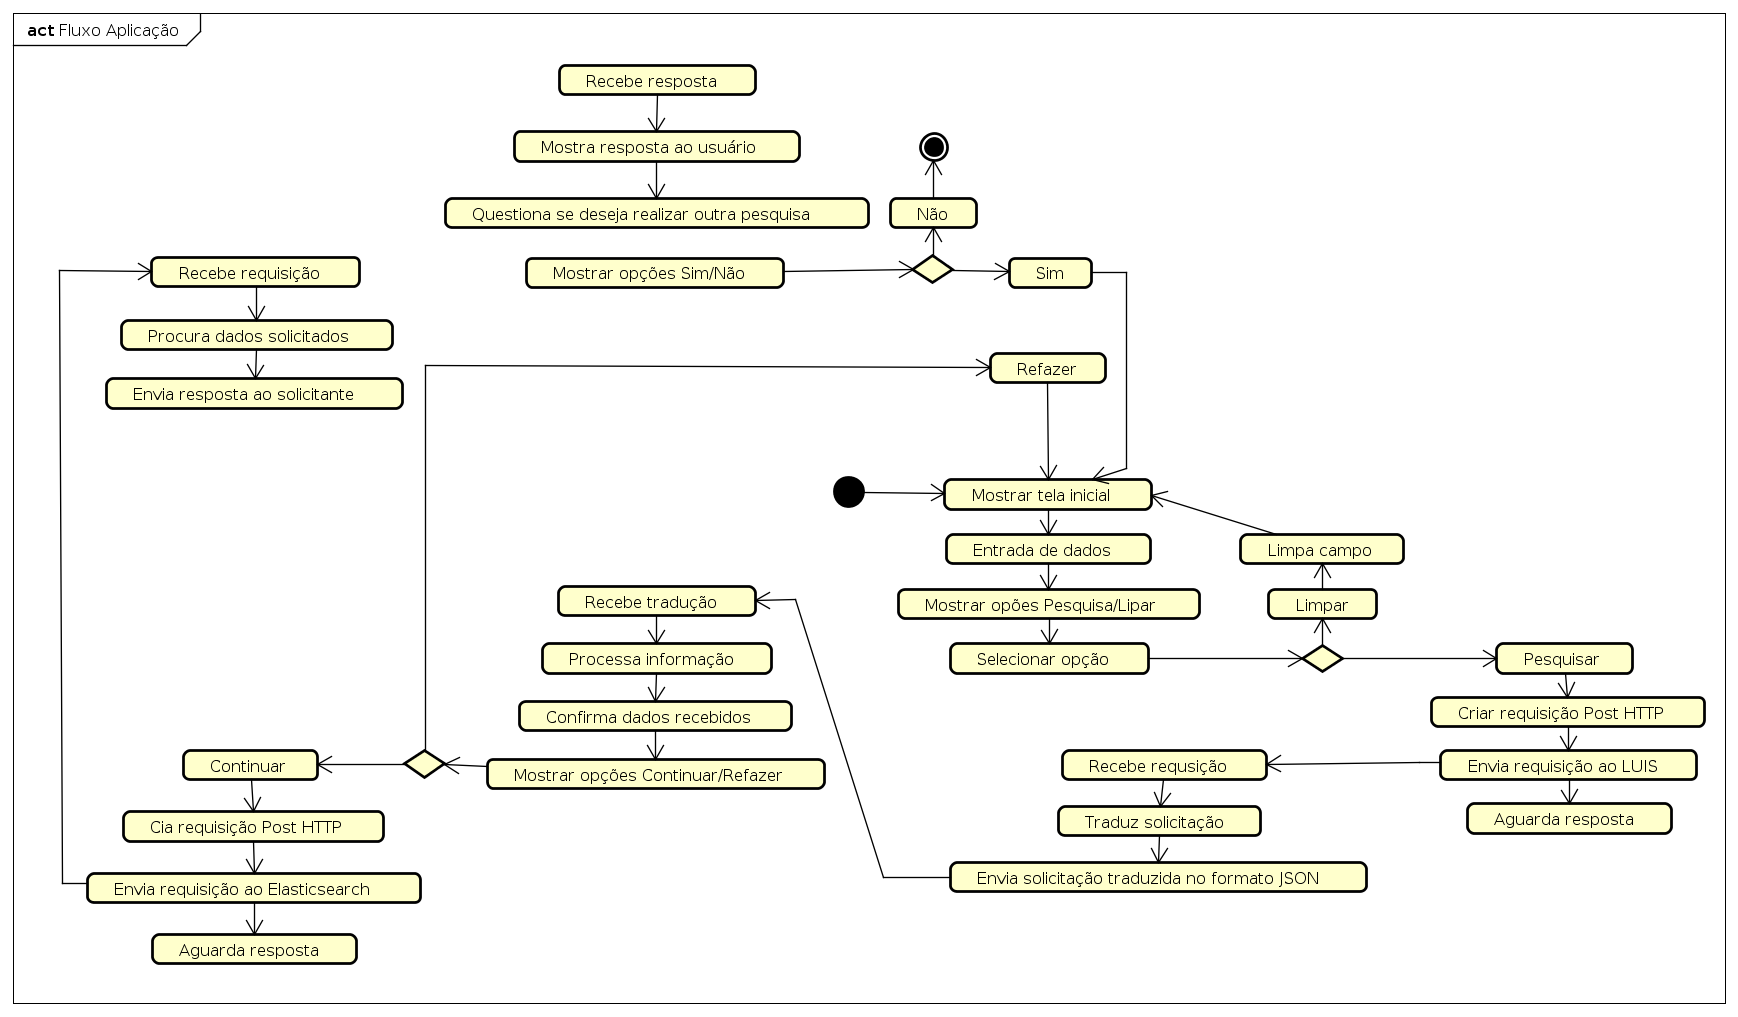
\includegraphics[angle=90, width=\textwidth, height=\textheight]{imagens/teste1.eps}
		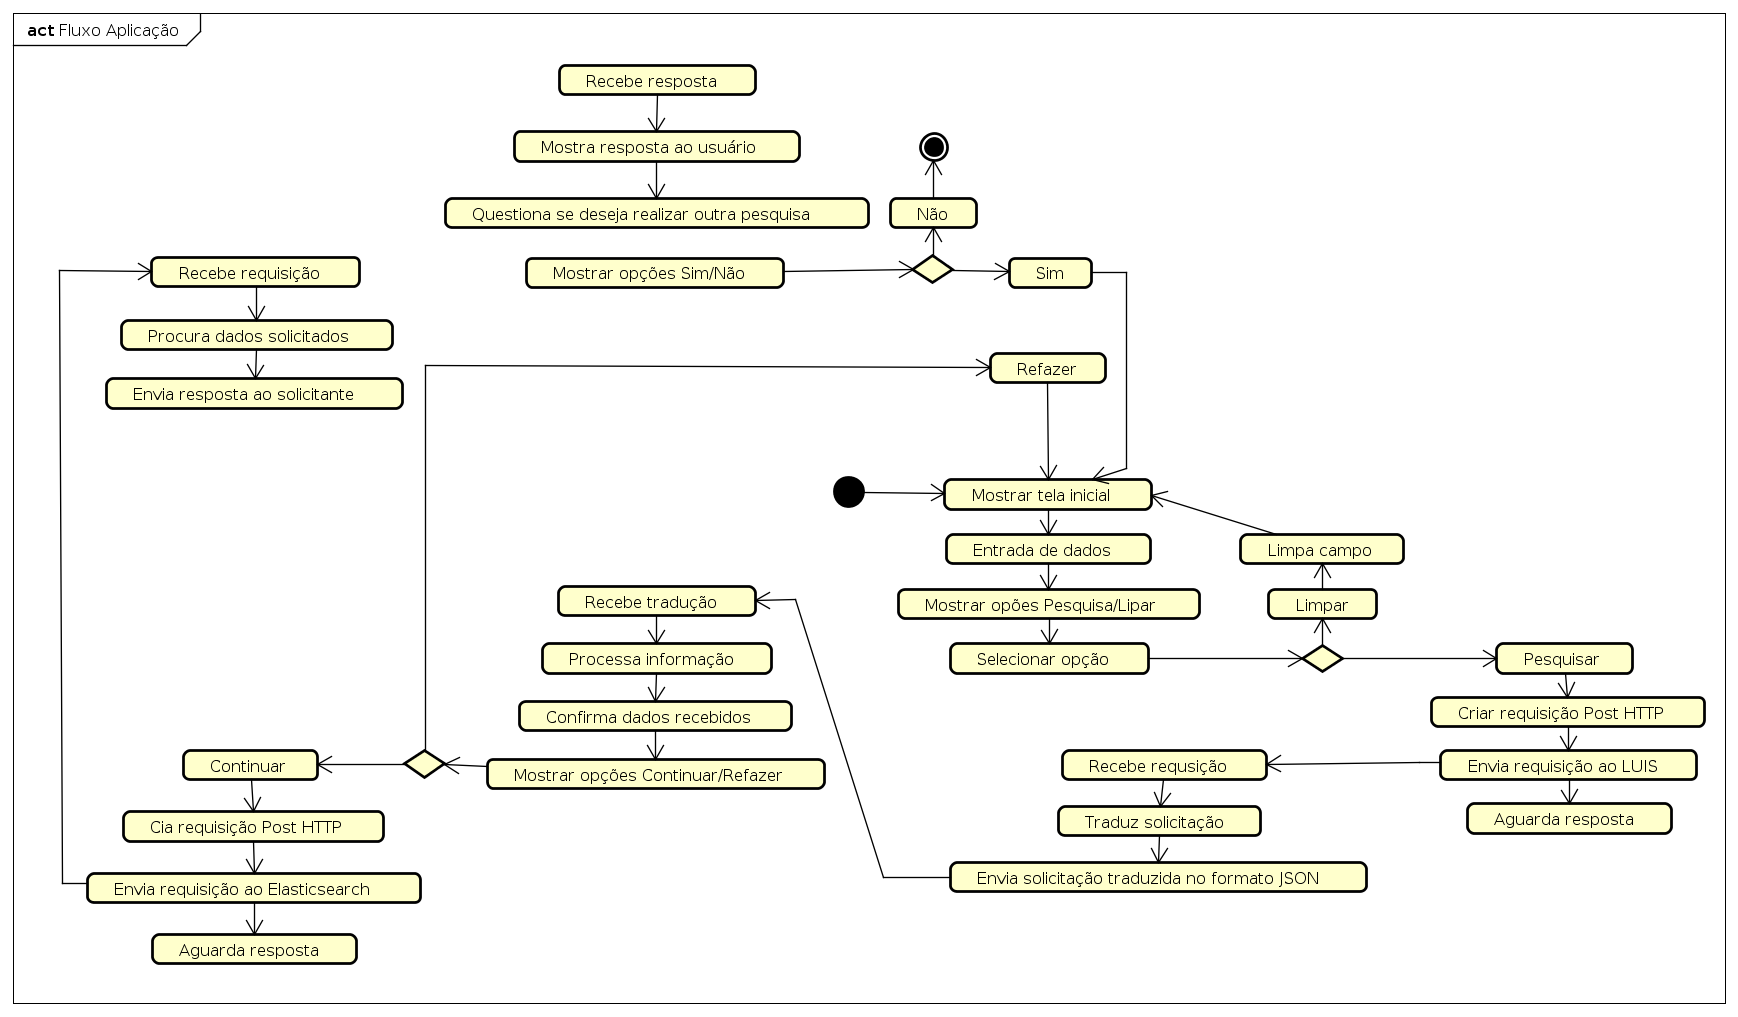
\includegraphics[width=0.5\textwidth, height=0.35\textheight]{imagens/diagfluxo.eps}
        \end{center}
        \legend{Fonte: Autor}
\end{figure}
